\begin{figure}[tb]
    \centering
    \begin{subfigure}[tb]{0.48\textwidth}
        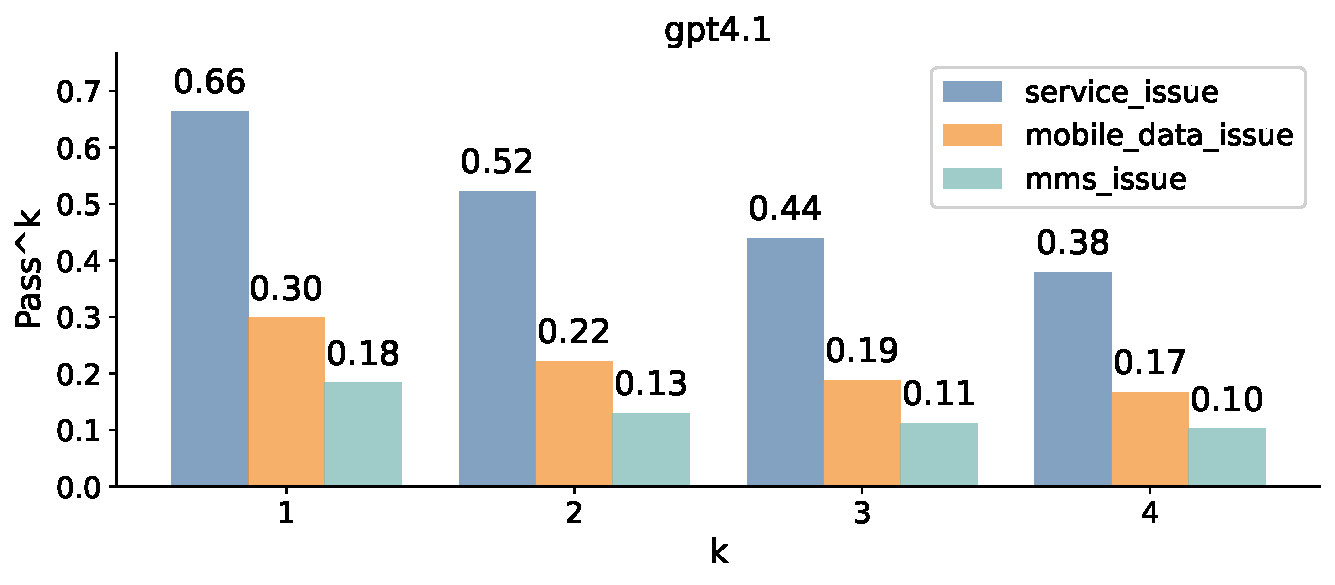
\includegraphics[width=\textwidth]{figures/results/pass_k_vs_k_per_intent_telecom_gpt-4.1-2025-04-14.pdf}
    \end{subfigure}
    \hfill
    \begin{subfigure}[tb]{0.48\textwidth}
        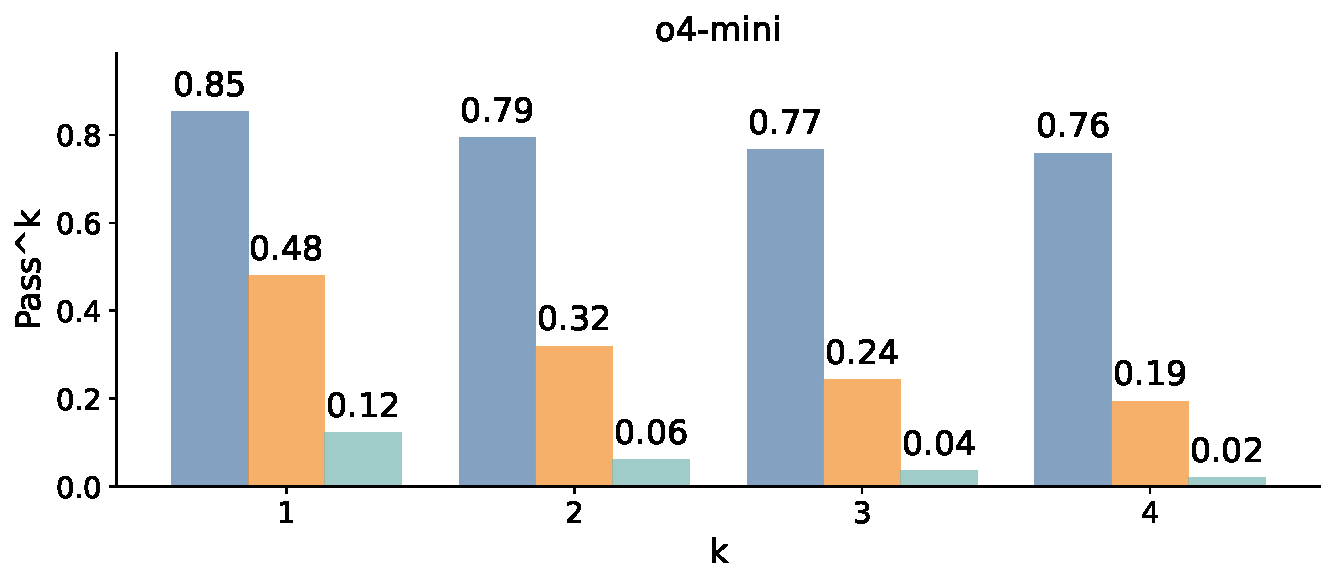
\includegraphics[width=\textwidth]{figures/results/pass_k_vs_k_per_intent_telecom_o4-mini-2025-04-16.pdf}
    \end{subfigure}
    \vspace{0.5em}
    \begin{subfigure}[tb]{0.48\textwidth}
        \centering
        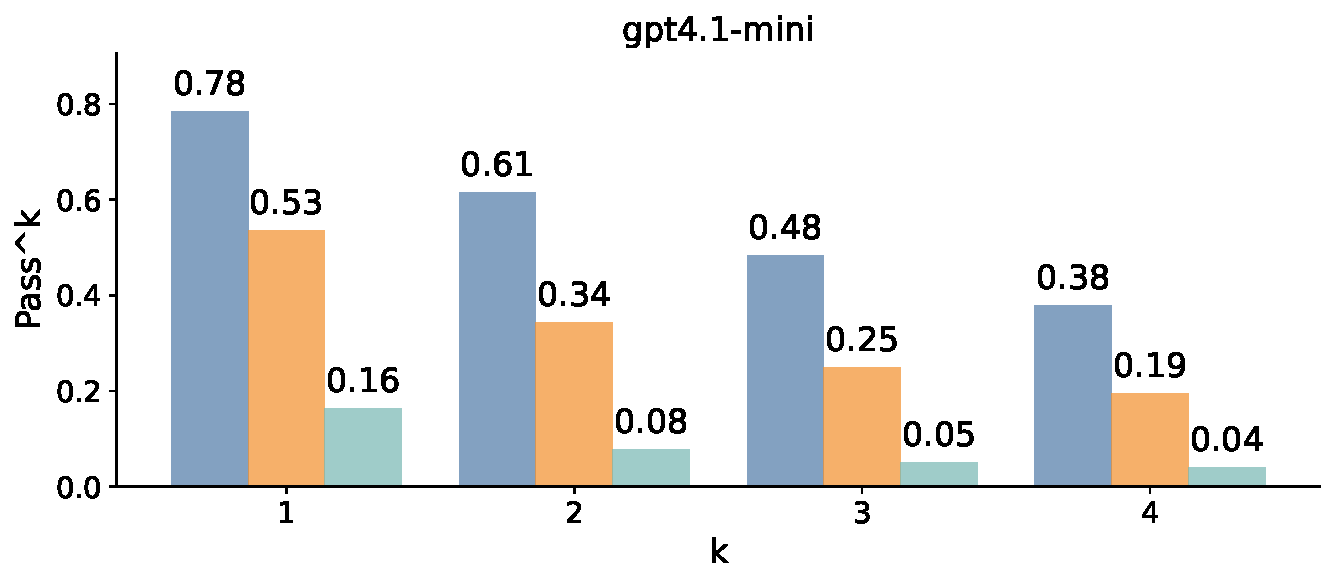
\includegraphics[width=\textwidth]{figures/results/pass_k_vs_k_per_intent_telecom_gpt-4.1-mini-2025-04-14.pdf}
    \end{subfigure}
    \hfill
    \begin{subfigure}[tb]{0.48\textwidth}
        \centering
        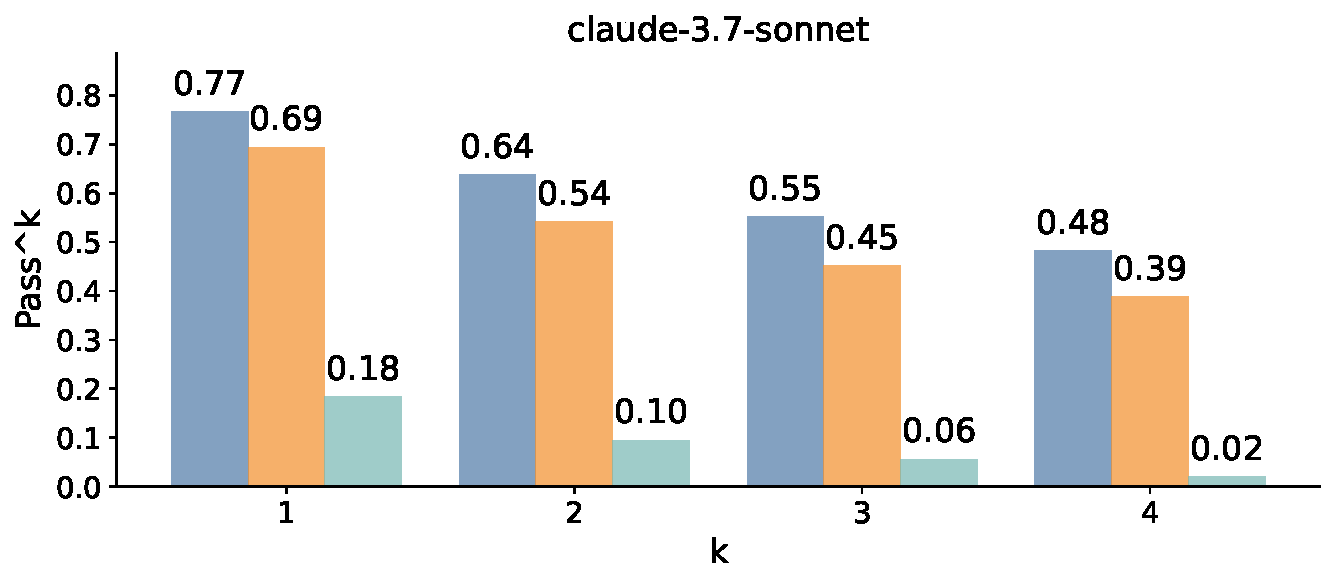
\includegraphics[width=\textwidth]{figures/results/pass_k_vs_k_per_intent_telecom_claude-3-7-sonnet-20250219.pdf}
    \end{subfigure}
    \vspace{-0.8em}
    \caption{\telecom 도메인에서 문제 유형별 \gptmodelshort(왼쪽 위), \ofourmodelshort(오른쪽 위), \gptminishort(왼쪽 아래), \claudesonnetshort(오른쪽 아래)의 \passk. \serviceissue, \mobiledataissue, \mmsissue 문제 유형에 대한 성능을 보여 주며, 서로 다른 문제 유형이 성공률에 어떤 영향을 미치는지 강조한다.}
    \label{fig:telecom_intent_results}
    \vspace{-1em}
\end{figure}

    
